\part{Rotating field theory}
\title[Rotating field theory]{Rotating field theory}  
\date{}  
\frame{\titlepage} 

%%%%%%%%%%%%%%%%%%%%%%%%%%%%%%%%%%%%%%%%%%%%%%%%%%%%%%%%%%%%%
%% Conceptual idea of a rotating magnetic field %%
%%%%%%%%%%%%%%%%%%%%%%%%%%%%%%%%%%%%%%%%%%%%%%%%%%%%%%%%%%%%%
\begin{frame}
	\frametitle{Conceptual idea of a rotating magnetic field}
    \begin{figure}
        \centering
        \movie{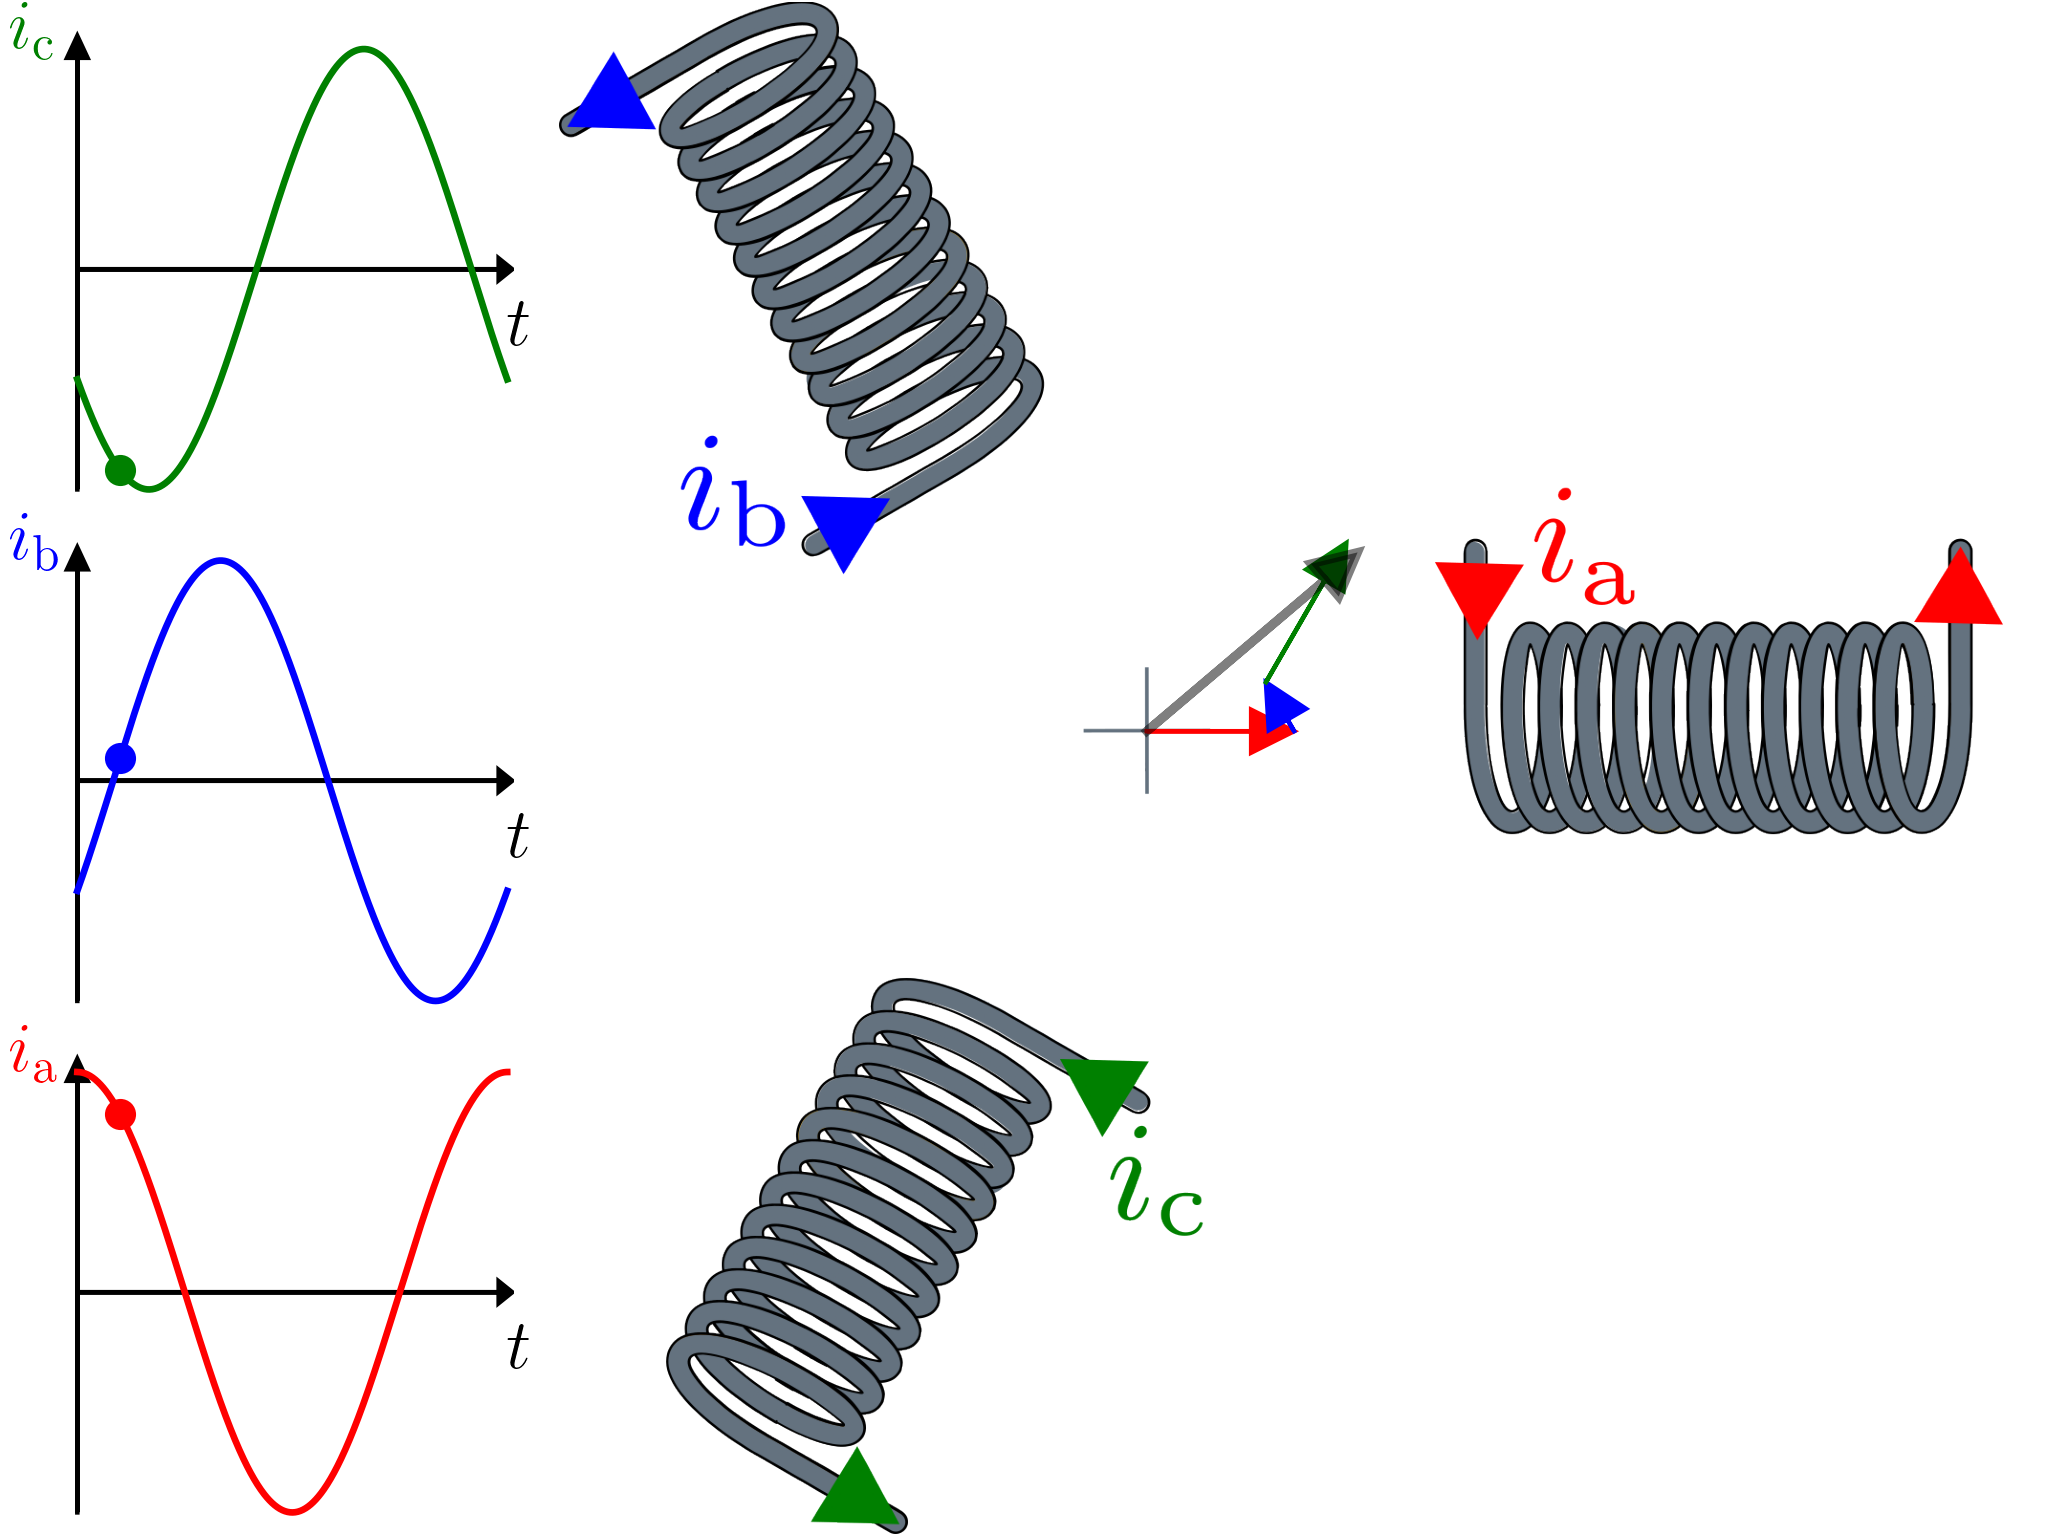
\includegraphics[height=0.7\textheight]{fig/lec05/Three_phase_coils_rotating_field_preview.png}}{fig/lec05/Three_phase_coils_rotating_field.gif}
        \caption{Animation of a rotating magnetic field produced by three-phase currents in three coils both physically and electrically displaced by $120^\circ$ (inspired by \href{https://perso.univ-lyon1.fr/charles.joubert/web_anim/simen_rotfield_create.html}{C.~Joubert})}
    \end{figure}
\end{frame}

%%%%%%%%%%%%%%%%%%%%%%%%%%%%%%%%%%%%%%%%%%%%%%%%%%%%%%%%%%%%%
%% MMF distribution of a single-phase coil %%
%%%%%%%%%%%%%%%%%%%%%%%%%%%%%%%%%%%%%%%%%%%%%%%%%%%%%%%%%%%%%
\begin{frame}
	\frametitle{MMF distribution of a single-phase coil}
			Utilizing Amp\`ere's law in the magnetic network context from \eqref{eq:ampere_law_magnetic_network}
            $$ \oint_{\partial S} \bm{H} \cdot \mathrm{d}\bm{s} = I_{\mathrm{f}} = N I = \sum_k  \theta_k = \sum_k l_k H_k $$
            and assuming that the air gap path along $\delta$ is dominating the magnetic circuit, we have
            \begin{equation}
                H(\vartheta) = \frac{1}{2\delta} \theta(\vartheta) = \frac{1}{2\delta} \begin{cases}
                    N i & \text{for } -\pi/2 \leq \vartheta < \pi/2, \\
                    -N i & \text{for } \pi/2 \leq \vartheta < 3\pi/2.
                \end{cases}
            \end{equation}
            \begin{figure}
                \begin{columns}
                    \begin{column}{0.5\textwidth}
                        \centering
                        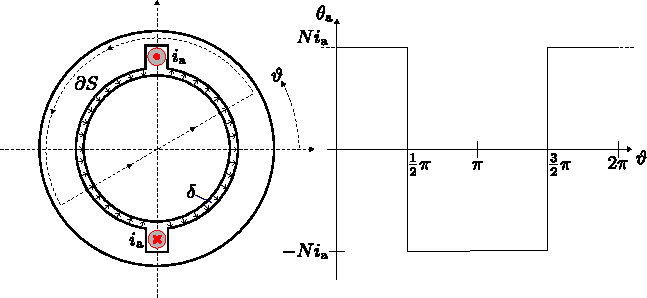
\includegraphics[width=\textwidth]{fig/lec05/MMF_single_phase.pdf}
                    \end{column}
                    \begin{column}{0.3\textwidth}
                        \caption{\raggedright MMF of a single-phase coil with $N$ turns for some current $i_\mathrm{a} \neq 0$ with the rotating integration path $\partial S$  along the circumference coordinate $\vartheta$}
				\label{fig: MMF_single_phase}
                    \end{column}
                \end{columns}
            \end{figure}
\end{frame}

%%%%%%%%%%%%%%%%%%%%%%%%%%%%%%%%%%%%%%%%%%%%%%%%%%%%%%%%%%%%%
%% Air gap flux density distribution of a single-phase coil %%
%%%%%%%%%%%%%%%%%%%%%%%%%%%%%%%%%%%%%%%%%%%%%%%%%%%%%%%%%%%%%
\begin{frame}
	\frametitle{Air gap flux density distribution of a single-phase coil}
    With $B=\mu_0 H$ in the air gap and an alternating current $i = i_\mathrm{a}(t)$, we have
    \begin{equation}
        B(\vartheta, t) = \frac{\mu_0}{2\delta} \begin{cases}
            N i_\mathrm{a}(t) & \text{for } -\pi/2 \leq \vartheta < \pi/2, \\
            -N i_\mathrm{a}(t) & \text{for } \pi/2 \leq \vartheta < 3\pi/2.
        \end{cases}
    \end{equation}
    \begin{figure}
        \begin{columns}
            \begin{column}{0.7\textwidth}
                \centering
		\begin{subfigure}[b]{0.45\textwidth}
			\centering
			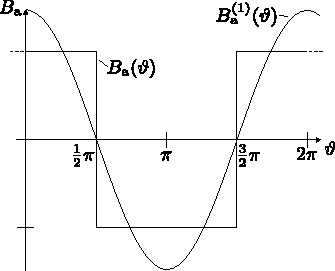
\includegraphics[width=\textwidth]{fig/lec05/B_single_phase_full_current.pdf}
			\caption{$i_\mathrm{a}(t) = \hat{i}$}
		\end{subfigure}
		\hfill
		\begin{subfigure}[b]{0.45\textwidth}
			\centering
			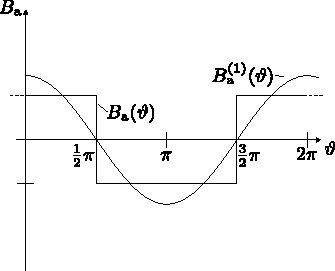
\includegraphics[width=\textwidth]{fig/lec05/B_single_phase_half_current.pdf}
			\caption{$i_\mathrm{a}(t) = \hat{i}/2$}
		\end{subfigure}
            \end{column}
            \begin{column}{0.3\textwidth}
                \caption{Air gap flux density distribution of a single-phase coil representing a spatiotemperal function} 
        \label{fig:Air_gap_flux_density_single_phase_coil}
            \end{column}
        \end{columns}
	\end{figure}
\end{frame}

%%%%%%%%%%%%%%%%%%%%%%%%%%%%%%%%%%%%%%%%%%%%%%%%%%%%%%%%%%%%%
%% Fourier analysis of the air gap flux density distribution %%
%%%%%%%%%%%%%%%%%%%%%%%%%%%%%%%%%%%%%%%%%%%%%%%%%%%%%%%%%%%%%
\begin{frame}
	\frametitle{Fourier analysis of the air gap flux density distribution}
        Assuming a sinusoidal current $i_\mathrm{a}(t) = \hat{i} \cos(\omega t)$, we have
        \begin{equation}
            B(\vartheta, t) = \underbrace{\frac{\mu_0 N \hat{i}}{2\delta}}_{\hat{B}} \begin{cases}
                \cos(\omega t) & \text{for } -\pi/2 \leq \vartheta < \pi/2, \\
                -\cos(\omega t) & \text{for } \pi/2 \leq \vartheta < 3\pi/2.
            \end{cases}
            \label{eq:B_single_phase_coil}
        \end{equation}
        The flux density distribution therefore is periodic and has a sinusoidal shape over $t$ as well as a rectangular shape over $\vartheta$. To anaylze the latter in terms of its fundamental and harmonic components, we utilize the Fourier series expansion for some arbitrary $t$:
        \begin{equation}
            B(\vartheta, t) =B(\vartheta) = \hat{B}^{(0)} + \sum_{k=1}^{\infty} \hat{B}_{\mathrm{c}}^{(k)} \cos(k \vartheta) + \hat{B}_{\mathrm{s}}^{(k)} \sin(k \vartheta),
            \label{eq:fourier_series_B_single_phase_coil}
        \end{equation} 
        for harmonic order $k=1,2,3,\ldots$ with amplitudes $\hat{B}_{\mathrm{c}}^{(k)}$ and $\hat{B}_{\mathrm{s}}^{(k)}$. 
\end{frame}

%%%%%%%%%%%%%%%%%%%%%%%%%%%%%%%%%%%%%%%%%%%%%%%%%%%%%%%%%%%%%
%% Fourier analysis of the air gap flux density distribution (cont.) %%
%%%%%%%%%%%%%%%%%%%%%%%%%%%%%%%%%%%%%%%%%%%%%%%%%%%%%%%%%%%%%
\begin{frame}
	\frametitle{Fourier analysis of the air gap flux density distribution (cont.)}
        The coefficients of \eqref{eq:fourier_series_B_single_phase_coil} are
        \begin{equation}
            \begin{split}
                \hat{B}^{(0)} &= \frac{1}{2\pi} \int_{0}^{2\pi} B(\vartheta) \mathrm{d}\vartheta, \\
                \hat{B}_{\mathrm{c}}^{(k)} &= \frac{1}{\pi} \int_{0}^{2 \pi} B(\vartheta) \cos(k \vartheta) \mathrm{d}\vartheta, \\
                \hat{B}_{\mathrm{s}}^{(k)} &= \frac{1}{\pi} \int_{0}^{2\pi} B(\vartheta) \sin(k \vartheta) \mathrm{d}\vartheta.
            \end{split}
        \end{equation}
        For an ideal symmetrical motor and a 180$^\circ$ shifted winding configuration as in \figref{fig: MMF_single_phase}, the magnetic field does not have any offset component:
        $$\hat{B}^{(0)} = 0.$$ Furthermore, \eqref{eq:B_single_phase_coil} is an even function, i.e., $B(\vartheta)=B(-\vartheta)$ (i.e., the function is mirror-symmetrical to the $\vartheta$ axis -- cf. \figref{fig:Air_gap_flux_density_single_phase_coil}), leading to $$\hat{B}_{\mathrm{s}}^{(k)} = 0.$$
\end{frame}

%%%%%%%%%%%%%%%%%%%%%%%%%%%%%%%%%%%%%%%%%%%%%%%%%%%%%%%%%%%%%
%% Fourier analysis of the air gap flux density distribution (cont.) %%
%%%%%%%%%%%%%%%%%%%%%%%%%%%%%%%%%%%%%%%%%%%%%%%%%%%%%%%%%%%%%
\begin{frame}
	\frametitle{Fourier analysis of the air gap flux density distribution (cont.)}
        Finally, \eqref{eq:B_single_phase_coil} is symmetrical w.r.t. the abscissa, i.e., $B(\vartheta)=-B(\vartheta+\pi)$ (mirrored positive and negative half-wave), leading to
        $$\hat{B}_{\mathrm{c}}^{(k)} = 0 \quad \mbox{for } \quad k=2,4,5,\ldots .$$
        Summarizing the above, the Fourier series for the air gap flux density boils down to
        \begin{equation}
            B(\vartheta) = \sum_{k=1,3,5,\ldots}^{\infty} \hat{B}_{\mathrm{c}}^{(k)} \cos(k \vartheta) \quad \mbox{with} \quad \hat{B}_{\mathrm{c}}^{(k)} = \frac{1}{\pi} \int_{0}^{2 \pi} B(\vartheta) \cos(k \vartheta) \mathrm{d}\vartheta.
            \label{eq:fourier_series_B_single_phase_coil_reduced}
        \end{equation}
        Utilizing symmetry of we can calculate $\hat{B}_{\mathrm{c}}^{(k)}$ for $k=1,3,5,\ldots$ as follows:
        \begin{equation}
            \begin{split}
                \hat{B}_{\mathrm{c}}^{(k)} &= \frac{2}{\pi} \int_{-\pi/2}^{\pi/2} B(\vartheta) \cos(k \vartheta) \mathrm{d}\vartheta = \frac{\mu_0 N \hat{i}}{\delta \pi } \cos(\omega t) \int_{-\pi/2}^{\pi/2} \cos(k \vartheta) \mathrm{d}\vartheta \\ &= \frac{\mu_0 N \hat{i}}{k \delta \pi } \cos(\omega t) \left[ \sin(\frac{k \pi}{2}) - \sin(-\frac{k \pi}{2}) \right] = \frac{2 \mu_0 N \hat{i}}{\delta \pi k} \cos(\omega t) \sin(\frac{k \pi}{2}).
            \end{split}
        \end{equation}
\end{frame}

%%%%%%%%%%%%%%%%%%%%%%%%%%%%%%%%%%%%%%%%%%%%%%%%%%%%%%%%%%%%%
%% Fourier analysis of the air gap flux density distribution (cont.) %%
%%%%%%%%%%%%%%%%%%%%%%%%%%%%%%%%%%%%%%%%%%%%%%%%%%%%%%%%%%%%%
\begin{frame}
	\frametitle{Fourier analysis of the air gap flux density distribution (cont.)}
    \begin{columns}
		\begin{column}{0.57\textwidth}
	        The Fourier series describing the spatiotemperal air gap flux density distribution of a single-phase coil from \eqref{eq:B_single_phase_coil} is therefore
        \begin{equation}
            \begin{split}
                B(\vartheta, t) &= \frac{2 \mu_0 N \hat{i}}{\delta \pi}\cos(\omega t)\sum_{k=1,3,5,\ldots}^{\infty}   \frac{1}{k}\sin(\frac{k \pi}{2})\\ &= \frac{4}{\pi} \hat{B} \cos(\omega t)\sum_{k=1,3,5,\ldots}^{\infty}   \frac{1}{k}\sin(\frac{k \pi}{2}).
            \end{split}
            \label{eq:fourier_series_B_single_phase_coil_final}
        \end{equation}
        Hence, the fundamental component $\hat{B}^{(1)}$ of the air gap flux density distribution is $4/\pi$ times higher than the amplitude $\hat{B}$ of the original square wave function from \eqref{eq:B_single_phase_coil} while the harmonic amplitude decrease with $1/k$. 
        \end{column}
        \begin{column}{0.43\textwidth}
            \begin{figure}
                \centering
                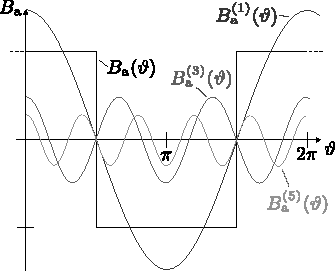
\includegraphics[width=\textwidth]{fig/lec05/B_single_phase_harmonics.pdf}
                \caption{Decomposition of $B(\vartheta, t)$ for some arbitrary $t$ into its fundamental and its first two harmonic components}
                \label{fig:B_single_phase_harmonics}
            \end{figure}
        \end{column}
    \end{columns}
\end{frame}

%%%%%%%%%%%%%%%%%%%%%%%%%%%%%%%%%%%%%%%%%%%%%%%%%%%%%%%%%%%%%
%% Remark on harmonics and multipole stators %%
%%%%%%%%%%%%%%%%%%%%%%%%%%%%%%%%%%%%%%%%%%%%%%%%%%%%%%%%%%%%%
\begin{frame}
	\frametitle{Remark on harmonics and multipole stators}
    \begin{varblock}{Flux density harmonics}
        The existence of harmonics is to be attributed to the spatial distribution of the winding. The phase current was assumed to be of pure sinusoidal form, i.e., is not causing the flux density harmonics.
    \end{varblock}
\end{frame}

%%%%%%%%%%%%%%%%%%%%%%%%%%%%%%%%%%%%%%%%%%%%%%%%%%%%%%%%%%%%%
%% Basic rotating field model %%
%%%%%%%%%%%%%%%%%%%%%%%%%%%%%%%%%%%%%%%%%%%%%%%%%%%%%%%%%%%%%
\begin{frame}
	\frametitle{Basic rotating field model}
    \begin{columns}
		\begin{column}{0.55\textwidth}
	        We assume an ideal three-phase stator current:
            \begin{equation}
                \begin{split}
                    i_\mathrm{s,a}(t) &= \hat{i}_{\mathrm{s}} \cos(\omega t), \\
                    i_\mathrm{s,b}(t) &= \hat{i}_{\mathrm{s}} \cos(\omega t - 2\pi/3), \\
                    i_\mathrm{s,c}(t) &= \hat{i}_{\mathrm{s}} \cos(\omega t + 2\pi/3).
                \end{split}
            \end{equation}
            The index 's' indicates stator quantities, but is omitted in the following as we will only consider stator quantities until further notice, i.e.,, 
            $$i_\mathrm{s,a}(t) = i_\mathrm{a}(t), \quad i_\mathrm{s,b}(t) = i_\mathrm{b}(t), \quad i_\mathrm{s,c}(t) = i_\mathrm{c}(t)$$
            and $\hat{i}_{\mathrm{s}}=\hat{i}$. 
        \end{column}
        \begin{column}{0.45\textwidth}
            \begin{figure}
                \centering
                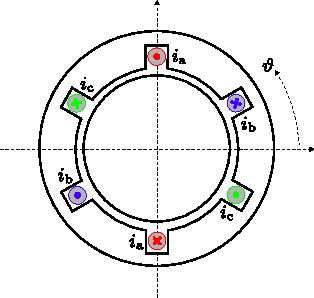
\includegraphics[width=0.8\textwidth]{fig/lec05/Simple_three_phase_stator_lumped_coils.pdf}
                \caption{Elementary three-phase stator winding with lumped coils  displaced by $120^\circ$. The rotor is considered an unspecific solid dummy with very high magnetic permeability.}
                \label{fig:Simple_three_phase_stator_lumped_coils}
            \end{figure}
        \end{column}
    \end{columns}
\end{frame}